\subsection{Funktionen}
    Die Aufgabe des Annotator Plugins besteht aus zwei Teilen.
    Zum einen soll sie die Klasse eines Features visualisieren
    und zum anderen soll es diese Klasse durch den Nutzer editierbar machen.

    Die Visualisierung besteht aus zwei Teilen und ist in Abbildung
    \ref{image:annotatorPluginViewer} dargestellt.

    \begin{figure}[htb]
        \centering
        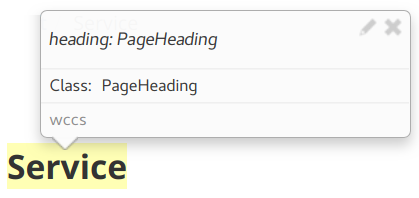
\includegraphics[width=0.5\textwidth]{../resources/annotator-plugin/viewer.png}
        \caption{Ergänzung des Annotation Viewers}
        \label{image:annotatorPluginViewer}
    \end{figure}

    Der Name der Klasse ist im Text der Annotation
    enthalten\footnote{vgl. Kapitel \ref{section:solutionDetailsAnnotationServiceFunctions}}.
    Der Nutzer kann diesen Text editieren.
    Diese Änderung wird zwar nicht
    persistiert\footnote{vgl. Kapitel \ref{section:solutionDetailsAnnotationServiceMapping}}
    ist aber in der Annotation bis zum Neuladen der Seite sichtbar.
    Aus diesem Grund wird die Klasse nochmals in einem zweiten Feld angezeigt,
    welches durch das Plugin ergänzt und auf Basis des Feldes
    "`wccs.featureClass"'\footnote{vlg. Kapitel \ref{section:solutionDetailsAnnotationServiceFunctions}}
    in der Annotation befüllt wird.

    Beim Editoeren wird dieser Bereich zu einer Auswahlliste,
    wie Abbildung \ref{image:annotatorPluginEditor} zeigt.

    \begin{figure}[htb]
        \centering
        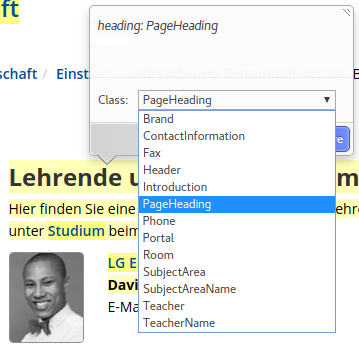
\includegraphics[width=0.5\textwidth]{../resources/annotator-plugin/editor.png}
        \caption{Ergänzung des Annotation Editors}
        \label{image:annotatorPluginEditor}
    \end{figure}

    Der Nutzer erhält dadurch die Möglichkeit die Klasse des Features zu bearbeiten.
    Die Einträge der Auswahlliste sind je nachdem,
    ob es sich um ein Content oder ein Reference Feature handelt,
    Inhalts- oder Referenzklassen.
    Diese Information wird aus dem Feld "`wccs.featureKind"' der Annotation bezogen.
    Die Klassen werden beim Initialisieren des Plugins einmalig beim
    Classification Service angefragt\footnote{vgl. Kapitel \ref{section:solutionDetailsClassificationServiceFunctions}}.
    Beim Speichern der Annotation wird die ausgewählte Klasse im Feld "`wccs.featureClass"' gespeichert,
    welches im Anschluss vom Annotation Service ausgelesen
    wird\footnote{vgl. Kapitel \ref{section:solutionDetailsAnnotationServiceMapping}}.
